\chapter{Planificación}

Para abordar las limitaciones discutidas en el apartado anterior, se desarrollará HangOut, una aplicación móvil innovadora diseñada específicamente para ayudar a las personas a descubrir establecimientos y eventos que se alineen con sus intereses personales. HangOut integrará y mejorará las funcionalidades de las plataformas existentes con características avanzadas que incluyen:

\begin{enumerate}
    \item \textbf{Centralización de la Información:} HangOut centraliza la información de diversos establecimientos y eventos, permitiendo al usuario encontrar rápidamente opciones que se ajusten a sus preferencias sin necesidad de consultar múltiples fuentes.

    \item \textbf{Interacción y Organización Social:} La aplicación permite a los usuarios seguir a otros, crear actividades y organizar salidas grupales de manera más eficiente, eliminando la necesidad de coordinarse a través de múltiples aplicaciones de mensajería.

    \item \textbf{Herramientas para Administradores de Establecimiento:} HangOut proporciona a los administradores una plataforma para gestionar sus perfiles de establecimiento indicando el ambiente, eventos y ofertas, facilitando así la promoción y gestión de sus servicios de manera más eficaz.

    \item \textbf{Enfoque Exclusivo:} La aplicación se distingue por su enfoque exclusivo en el ocio y la eficiencia en la organización de eventos. Combinando la funcionalidad de creaciones de actividades en grupos específicos con la búsqueda de establecimientos y la personalización según las preferencias del usuario, ofreciendo una solución más específica para el ocio.
\end{enumerate}

\section{Metodología de Desarrollo Ágil}

Las metodologías ágiles de desarrollo de software son ampliamente utilizadas hoy en día debido a su alta flexibilidad y capacidad de adaptación. Estas metodologías permiten a los equipos de trabajo ser más productivos y eficientes, ya que tienen claridad sobre las tareas durante el desarrollo. En el proceso, el software se va adaptando a las nuevas necesidades y requerimientos que vayan surgiendo, facilitando la creación de aplicaciones funcionales \cite{santander}.

Este tipo de metodologías de desarrollo tienen ciertas características claves que hace que destaque respecto a las tradicionales:

\begin{enumerate}
    \item \textbf{Flexibilidad y Agilidad:} Permiten la adaptación continua del software a medida que se identifican nuevas necesidades por parte de los usuarios.

    \item \textbf{Desarrollo Incremental:} En cada ciclo de desarrollo se van agregando nuevas funcionalidades.

    \item \textbf{Ciclos de Desarrollo Cortos:} Los ciclos de desarrollo, conocidos como iteraciones o sprints, son cortos y permiten la entrega continua de incremento funcionales del software, facilitando un feedback continuo.
\end{enumerate}

\subsection{Ejemplos de Metodologías}

\begin{enumerate}
    \item \textbf{Kanban:} Se basa en dividir las tareas en porciones más pequeñas y organizarlas en un tablero de trabajo con columnas de tareas pendientes, en curso y finalizadas. Este sistema crea un flujo de trabajo visual que ayuda a priorizar las tareas y mejorar el valor del producto.

          \begin{figure}[H]
              \centering
              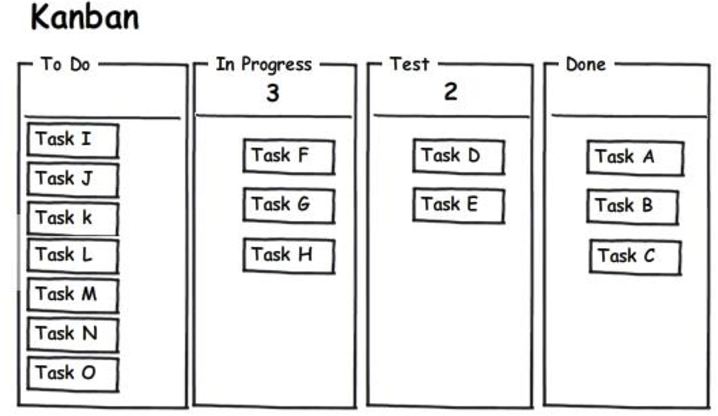
\includegraphics[width=0.5\textwidth]{imagenes/Kanban.png}
              \caption{Kanban \cite{kanban_img}}
              \label{fig:kanban}
          \end{figure}

    \item \textbf{Scrum:} Es una metodología incremental que organiza los requisitos y tareas en ciclos cortos y fijos, denominados sprints. Las etapas incluyen la planificación del sprint, ejecución, reuniones diarias y revisión de los resultados. Cada iteración completa estas etapas, permitiendo entregar un producto funcional al final de cada sprint.

          \begin{figure}[H]
              \centering
              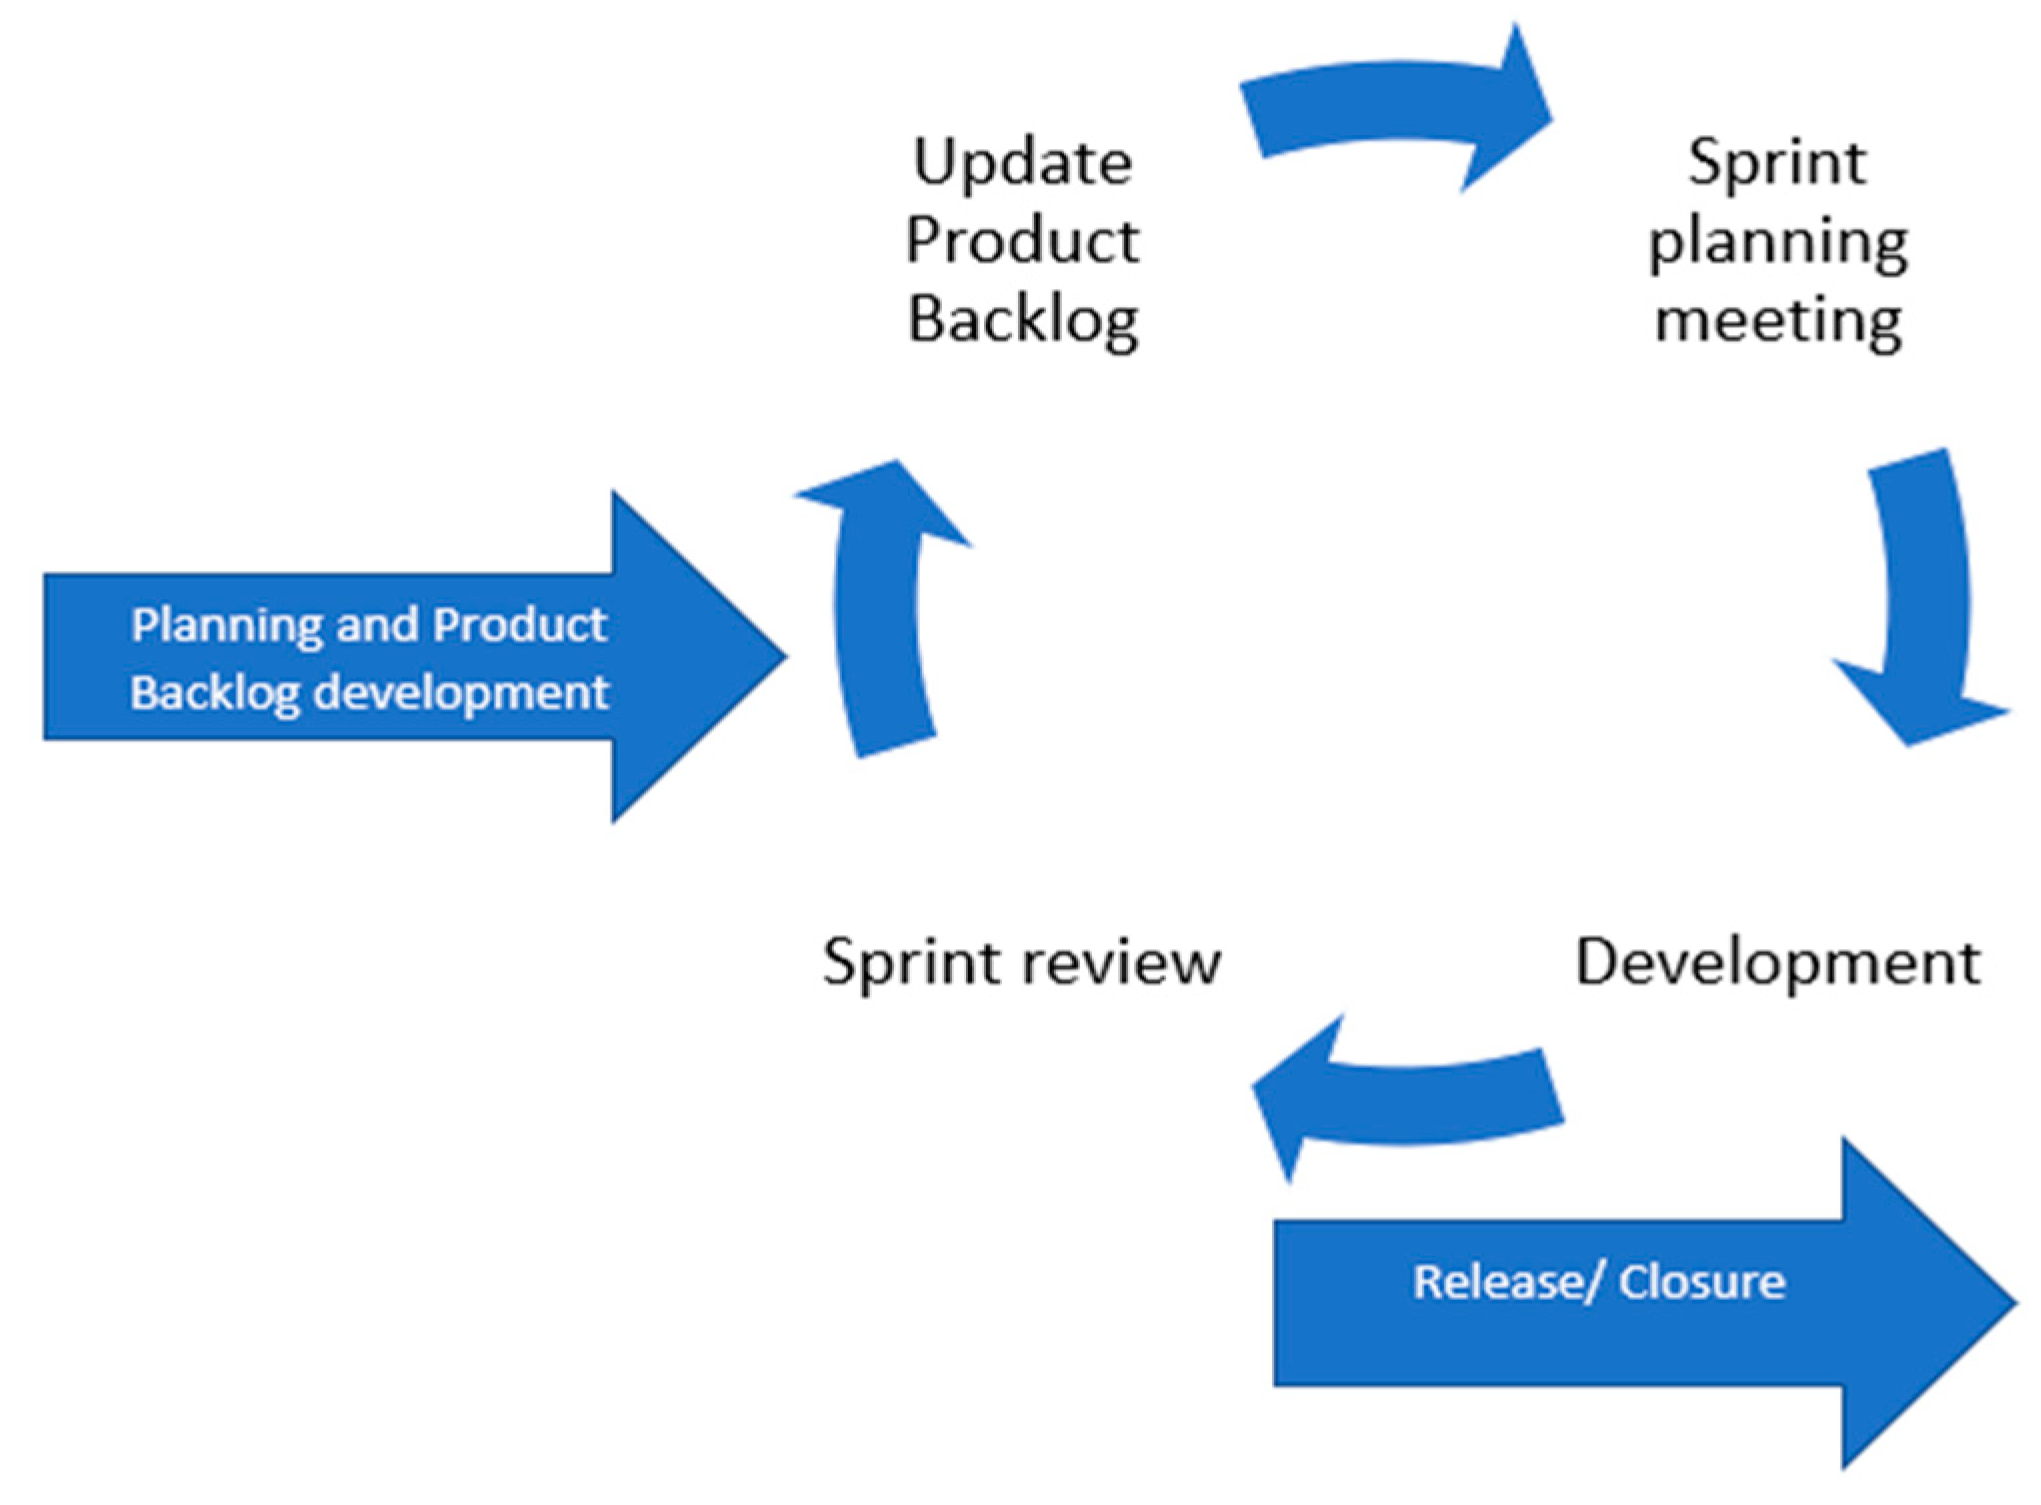
\includegraphics[width=0.5\textwidth]{imagenes/Scrum.jpg}
              \caption{Scrum \cite{scrum_img}}
              \label{fig:scrum}
          \end{figure}

    \item \textbf{Lean:} Enfocada en equipos pequeños y altamente capacitados, promueve la rápida ejecución de tareas y valora principalmente el compromiso y la capacidad de aprendizaje del equipo. Los ciclos cortos permiten adaptarse rápidamente a los cambios y mejorar el producto.

          \begin{figure}[H]
              \centering
              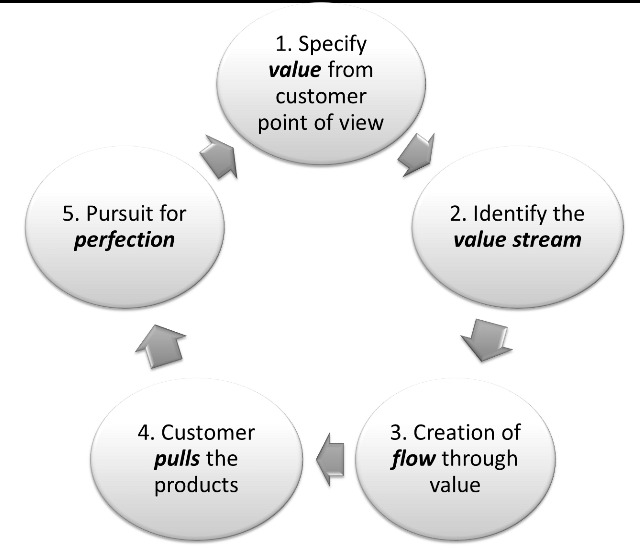
\includegraphics[width=0.5\textwidth]{imagenes/Lean.jpg}
              \caption{Scrum \cite{lean_img}}
              \label{fig:lean}
          \end{figure}

\end{enumerate}

Para llevar a cabo mi proyecto, decidí utilizar una metodología de desarrollo ágil como es \textbf{Scrum}. Esta elección fue motivada por diferentes razones con el objetivo de maximizar la eficiencia y calidad del producto final. Los principales motivos fueron:

\begin{enumerate}
    \item \textbf{Adaptación a Cambios Continuos:} Al desempeñar el rol de programador y usuario de la aplicación la capacidad de adaptación se volvió un papel muy importante, los requisitos podían cambiar a medida que avanzaba el desarrollo. Utilizando Scrum, con sus sprints cortos y revisiones frecuentes, me permitió ajustar el rumbo del proyecto ágilmente.

    \item \textbf{Desarrollo Incremental:} Me permitió dividir el trabajo en partes manejables y poder completar incrementos funcionales del software de manera continua. Cada sprint incluía la implementación y prueba de nuevas funcionalidades.

    \item \textbf{Mejora Continua:} Aunque trabajé de forma independiente, seguí prácticas de Scrum como revisiones de sprint para mantener la organización del proyecto. Adicionalmente, me reunía cada cierto tiempo con mi tutor para poder revisar mi avance.

\end{enumerate}

\begin{figure}[H]
    \centering
    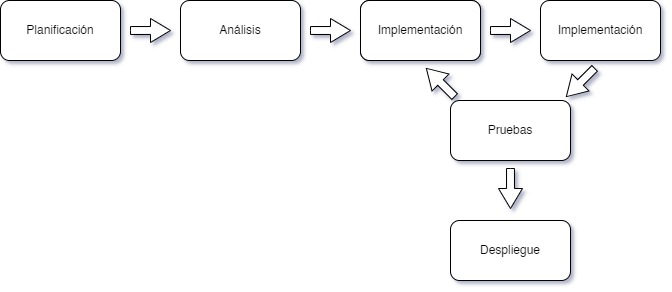
\includegraphics[width=0.5\textwidth]{imagenes/DiagramaEtapas.jpg}
    \caption{Diagrama de las etapas del proyecto}
    \label{fig:diagrama_etapas}
\end{figure}


\section{Cronograma y Planificación}

El proyecto comenzó a mitad de febrero de 2024, con la meta de ser completado a finales de junio del mismo año. Para visualizar la planificación del mismo, se presenta un Diagrama de Gantt. Este diagrama es una representación gráfica del cronograma del proyecto, donde las tareas se describen en el  eje vertical y el tiempo empleado en cada una de ellas en el eje horizontal. El diagrama muestra las fechas de inicio y finalización del proyecto, facilitando el seguimiento y la gestión de las distintas etapas del desarrollo.

La aplicación se ha desarrollado utilizando tecnologías como Python y React Native, de las cuales no tenía experiencia previa. Por lo tanto, la planificación del proyecto se realizó teniendo en cuenta el tiempo necesario para aprender y familiarizarme con estos lenguajes. Este proceso incluyó la dedicación del tiempo adicional para la formación y la práctica de ambas tecnologías, asegurando así un desarrollo ágil y eficiente de la aplicación.

\subsection{Diagrama de Gantt}

El desarrollo completo de la aplicación se extendió a lo largo de cuatro meses. Durante este período, se abordaron diversas etapas del proceso de desarrollo, las cuales se detallan en el siguiente diagrama de Gantt. Este diagrama ofrece una representación visual detallada del cronograma del proyecto, desglosando cada una de las etapas.

\begin{figure}[H]
    \centering
    \scriptsize
    \resizebox{\textwidth}{!}{%
        \begin{ganttchart}[
                hgrid,
                vgrid={*{6}{draw=none}, dotted},
                title/.append style={fill=blue!10},
                title label font=\tiny,
                title height=1,
                bar/.append style={fill=gray!30},
                bar height=.4,
                y unit chart=0.7cm,
                x unit=0.2cm,
                time slot format=isodate,
                milestone left shift=-1,
                milestone right shift=2,
                group/.append style={draw=none, fill=none, font=\normalsize},
            ]{2024-02-16}{2024-06-24}

            \gantttitlecalendar{month=name} \\

            \ganttgroup[inline=false]{\textbf{\normalsize Investigación y Formación Inicial}}{2024-02-16}{2024-03-01} \\
            \ganttbar[name=python]{Estudio de Python y Flask}{2024-02-16}{2024-02-24} \\
            \ganttbar[name=react]{Estudio React Native}{2024-02-25}{2024-03-01} \\
            \ganttmilestone[name=fin_formacion]{Fin de Investigación y Formación}{2024-03-01} \\

            \ganttnewline

            \ganttgroup[inline=false]{\textbf{\normalsize Planificación del Proyecto}}{2024-03-01}{2024-03-09} \\
            \ganttbar[name=esquema]{Esquematizar el Proyecto}{2024-03-01}{2024-03-09} \\

            \ganttnewline

            \ganttgroup[inline=false]{\textbf{\normalsize Requisitos del Proyecto}}{2024-03-09}{2024-03-17} \\
            \ganttbar[name=req_func]{Requisitos Funcionales}{2024-03-09}{2024-03-14} \\
            \ganttbar[name=req_no_func]{Requisitos No Funcionales}{2024-03-15}{2024-03-17} \\

            \ganttnewline

            \ganttgroup[inline=false]{\textbf{\normalsize Diseño del Sistema}}{2024-03-17}{2024-03-31} \\
            \ganttbar[name=mockups]{Diseño de MockUps Iniciales}{2024-03-17}{2024-03-20} \\
            \ganttbar[name=db_design]{Diseño de Base de Datos}{2024-03-21}{2024-03-24} \\
            \ganttbar[name=uml]{Elaboración de Diagramas UML}{2024-03-25}{2024-03-31} \\
            \ganttmilestone[name=fin_diseno]{Fin de Diseño del Sistema}{2024-03-31} \\

            \ganttnewline

            \ganttgroup[inline=false]{\textbf{\normalsize Desarrollo del BackEnd}}{2024-04-01}{2024-04-30} \\
            \ganttbar[name=dev_env]{Configuración del Entorno de Desarrollo}{2024-04-01}{2024-04-03} \\
            \ganttbar[name=classes]{Implementación de Clases y Modelo}{2024-04-03}{2024-04-14} \\
            \ganttbar[name=api]{Implementación de EndPoints API}{2024-04-15}{2024-04-27} \\
            \ganttbar[name=postman]{Pruebas de EndPoint con POSTMAN}{2024-04-28}{2024-04-30} \\
            \ganttmilestone[name=fin_backend]{Fin de Desarrollo del BackEnd}{2024-04-30} \\

            \ganttnewline

            \ganttgroup[inline=false]{\textbf{\normalsize Desarrollo de FrontEnd}}{2024-05-01}{2024-06-06} \\
            \ganttbar[name=figma]{Diseño en Figma}{2024-05-01}{2024-05-04} \\
            \ganttbar[name=frontend_env]{Configuración del Entorno FrontEnd}{2024-05-04}{2024-05-07} \\
            \ganttbar[name=screens]{Desarrollo de Pantallas y Componentes}{2024-05-08}{2024-05-17} \\
            \ganttbar[name=expo]{Pruebas de Visualización en ExpoGo}{2024-05-17}{2024-05-18} \\
            \ganttbar[name=integration]{Integración del FrontEnd con BackEnd}{2024-05-19}{2024-05-25} \\
            \ganttbar[name=navigation]{Implementación de Navegación entre Pantallas}{2024-05-26}{2024-06-06} \\
            \ganttmilestone[name=fin_frontend]{Fin de Desarrollo del FrontEnd}{2024-06-06} \\

            \ganttnewline

            \ganttgroup[inline=false]{\textbf{\normalsize Documentación del Proyecto}}{2024-03-09}{2024-06-24} \\
            \ganttbar[name=doc]{Escritura de la Documentación}{2024-03-09}{2024-06-24} \\

            \ganttlink{react}{esquema}
            \ganttlink{esquema}{req_func}
            \ganttlink{req_func}{req_no_func}
            \ganttlink{req_no_func}{mockups}
            \ganttlink{mockups}{db_design}
            \ganttlink{db_design}{uml}
            \ganttlink{uml}{dev_env}
            \ganttlink{dev_env}{classes}
            \ganttlink{classes}{api}
            \ganttlink{api}{postman}
            \ganttlink{postman}{figma}
            \ganttlink{figma}{frontend_env}
            \ganttlink{frontend_env}{screens}
            \ganttlink{screens}{expo}
            \ganttlink{expo}{integration}
            \ganttlink{integration}{navigation}

        \end{ganttchart}
    }
    \caption{Diagrama de Gantt detallado con la planificación y fases de desarrollo}
    \label{fig:gantt_diagram_detailed}
\end{figure}




\section{Recursos y Materiales}

En este apartado se analizan los recursos y materiales utilizados durante el transcurso del proyecto.

\subsection{Recursos Humanos}

Para el desarrollo de la aplicación, el principal y único recurso humano he sido yo, ya que he desempeñado los roles de desarrollador y usuario. Además, es importante mencionar a mi tutor, quien me ha guiado a lo largo del proceso, proporcionando orientación y apoyo.

\subsection{Materiales}

Para el desarrollo del proyecto se ha utilizado un portátil personal y un segundo monitor, lo cual ha sido de gran ayuda a la hora de programar, permitiendo una mayor eficiencia y comodidad en la gestión de múltiples ventanas y herramientas. A parte de los materiales utilizados para el desarrollo también se ha utillzado un smartphone para la prueba del frontend utilizando la aplicación Expo Go:

\begin{enumerate}
    \item \textbf{Portátil:} ASUS TUF F15 FX506HC - Portátil de 15.6" Full HD 144Hz (Intel Core i5-11400H, 16GB RAM, 512GB SSD, NVIDIA RTX 3050-4GB). Con valor actual de 699.99 \EUR{} \cite{amazon_asus}

    \item \textbf{Monitor:} BenQ GW2480 - Monitor IPS LED de 23.8 Pulgadas 1080p. Con valor actual de 99.99 \EUR{} \cite{amazon_samsung}

    \item \textbf{Smartphone:} Samsung Galaxy S10e - Smartphone de 5.8”, Dual SIM, 128 GB. Con valor actual de 329.99 \EUR{} \cite{amazon_benq}
\end{enumerate}

\section{Presupuesto}

En este apartado se analiza y se describen los costes del proyecto utilizando información proporcionada por las bases de cotización para contingencias comunes del año 2024, según la Seguridad Social de España. El perfil será el de un ingeniero informático junior y teniendo en cuenta que las bases de cotización oscilan entre un mínimo de 1.847,40 \EUR{} y un máximo de 4.720,50 €. Se asumirá el uso de la base mínima de cotización y la duración de 5 meses del proyecto. \cite{seguridad_social}

Con esta información el coste total del salario para un ingeniero informático junior durante la duración del proyecto sería de
\[
    \textbf{Salario Informatico Junior} = 1\,847{,}40 \text{ \EUR{}/mes} \times 5 \text{ meses} = 9\,237 \text{\EUR{}}
\]


Si por su contraparte quisiéramos ver el coste total del salario para un ingeniero informático senior durante la duración del proyecto y utilizando el máximo de las bases de cotización mencionadas anteriormente, procederíamos de la siguiente manera:
\[
    \textbf{Salario Informatico Senior} = 4\,720{,}50 \text{ \EUR{}/mes} \times 5 \text{ meses} = 23\,602{,}50 \text{\EUR{}}
\]

Estas estimaciones no toman costes adicionales más allá de los descritos anteriormente.

En lo que respecta a las licencias para este proyecto, todas las tecnologías utilizadas han sido de código abierto con el fin de minimizar gastos. Como consecuencia a esta elección el coste total en licencias ha sido nulo.

Para estimar el coste del hardware mencionado en el apartado de materiales, es importante considerar la estimación de vida útil de un dispositivo, como puede ser un portátil o un smartphone, que es de 5 años.

\[
    \textbf{Coste Materiales} = 699{,}99 \text{ \EUR{}} + 329{,}99 \text{ \EUR{} } + 99{,}99 \text{ \EUR{}} = 1\,129{,}97 \text{ \EUR{}}
\]

\[
    \textbf{Coste Anual} = \frac{\text{Coste Material}}{5 \text{ años}} = 225{,}99 \text{ \EUR{}}
\]

\[
    \textbf{Coste Duración Proyecto} = \left( \frac{\text{Coste Anual}}{12 \text{ meses}} \right) \times 5 \text{ meses} = 94{,}16 \text{ \EUR{}}
\]

Sumando el coste del hardware al coste de los recursos humanos para un ingeniero informático junior, el coste total del proyecto durante estos 5 meses es de 9 331,16 \EUR{}. Para un ingeniero informático senior, el coste total del proyecto sería de 23 696,66 \EUR{}.

